%\documentclass[letterpaper, 10 pt, conference]{orbieeeconfpre}
%\conference{IEEE Conference for Awesome ORB Research}
\documentclass[a4paper, 10pt, journal]{wissarbIEEE}

\bibliographystyle{orbref-num}
\IEEEoverridecommandlockouts	%  defines \thanks command 
\overrideIEEEmargins			% Needed to meet printer requirements.

\usepackage{hyperref}
\usepackage{graphicx}
\usepackage{tabularx}
\usepackage{booktabs}

\title{\LARGE \bf Neural Networks for Tool Image Classification}

\author{Boas Bamberger $^{1}$, Oliver Erlenkaemper$^{2}$ and Fabian Wolf$^{3}$ 
\thanks{$^{1}$Boas Bamberger is with the Faculty for Business Studies, University of  Mannheim, L5 1, 68131 Mannheim {\tt\small bamberger@uni-mannheim.de}} \thanks{$^{2}$Oliver Erlenkaemper is with the Department for Research and Development, Movilizer GmbH, Konrad-Zuse-Ring 30, 68163 Mannheim {\tt\small oliver.erlenkaemper@honeywell.com}} \thanks{$^{3}$Fabian Wolf is with the Faculty for Business Informatics, Baden-Württemberg Cooperative State University (DHBW), Coblitzallee 1-9, 68163 Mannheim {\tt\small s172298@student.dhbw-mannheim.de}}
}


\begin{document}
%acronyms
% Tool Image Classification Dataset (TIC Dataset)
\maketitle
\begin{abstract}
TODO
\end{abstract}

\section{Introduction}

\section{Related Work}
TIC hat keiner gemacht, aber Image Classification ist großes Feld => Paper von verwendeten Modellen

\section{Method}
\label{sec:method}
Experiment: Modelle auf Dataset Trainieren und Testen (train, dev, test split)
Training Params in Tabell => Batchsize wurde an Ram Size angepasst, dataaugmentation, weight decay, dropout ist out of scope und wurde deshalb nicht verwendet, auch wenn es im original paper verwendet wurde
\subsection{Model Selection}
Models: Literaturreview nach Webster and Watsonn => meist verwendete Architekturen => Archetyp der Architektur
\subsection{Dataset Construction}
Dataset: Selbsterstellt (sphärisch um Objekt => verschiedene Winkel, verschiedene intergründe). 15.000, 6 klassen diese sind ..., diese sind balanciert (weil accuracy)

\section{Evaluation}
We evaluated the performance of the selected neural networks as described in Section \ref{sec:method}. The performances of the selected neural networks were measured in accuracy. The accuracy for each neural network is reported in Table \ref{tab:acc}. 
Among these neural networks, DenseNet-264 performs best for the {TIC Dataset}. ResNet-152, ResNeXt-101, and DenseNet-264 perform rather similar. Therefore, we conclude that several neural networks are suited for tool image classification.
\begin{table}[h]
\caption{Experiment Results} \label{tab:acc}
	\begin{tabularx}{0.48\textwidth}{Xc}
		\toprule 
		\textbf{Neural Network} & \textbf{Accuracy in $\%$} \\\midrule
		VGG-19 & $72.40$ \\
		ResNet-152 & $92.89$ \\
		ResNeXt-101 & $94.66$ \\
		\textbf{DenseNet-264} & $\mathbf{97.45}$ \\
		EfficientNet-B7 & $16.67$\\
		\bottomrule
	\end{tabularx}  \label{tab:initmodel}
\end{table}

\section{Discussion}
Verschiedene Modelle geeignet, 
DenseNet-264 best performing only under constraints of this paper (intro)
Several neural networks work for TIC => In accordance with related work

Despited differing in structure All use conv layer
Similar performing => Conv layers and skip con
VGG only conv performs worst => conv is the basis and skip cons boost performance

Efficient Net 16.67\% => just guessed, probably due to batchsize of one => loss function fluctuates heavily => impaired convergence

Komplette section Limitations

\section{Conclusion}
To the best of our knowledge we are the first to do tool image classification
zusammenfassung (several nns work for TIC, conv+skip con works good, practical implications: unsere modelle als basis für end2end impl des business scenarios)
verbesserungen (architecture search statt konkrete modelle, excluded learning auxiliaries, bigger batchsize for efficient net)
future work(more data, implement end2end business scenario)

\bibliography{mybibfile}
\end{document}

%================================EXAMPLES================================
% use \CITE
% use \section and \subsection, don't use \chapter

% Figure
%\begin{figure}[h]
%   \centering
%   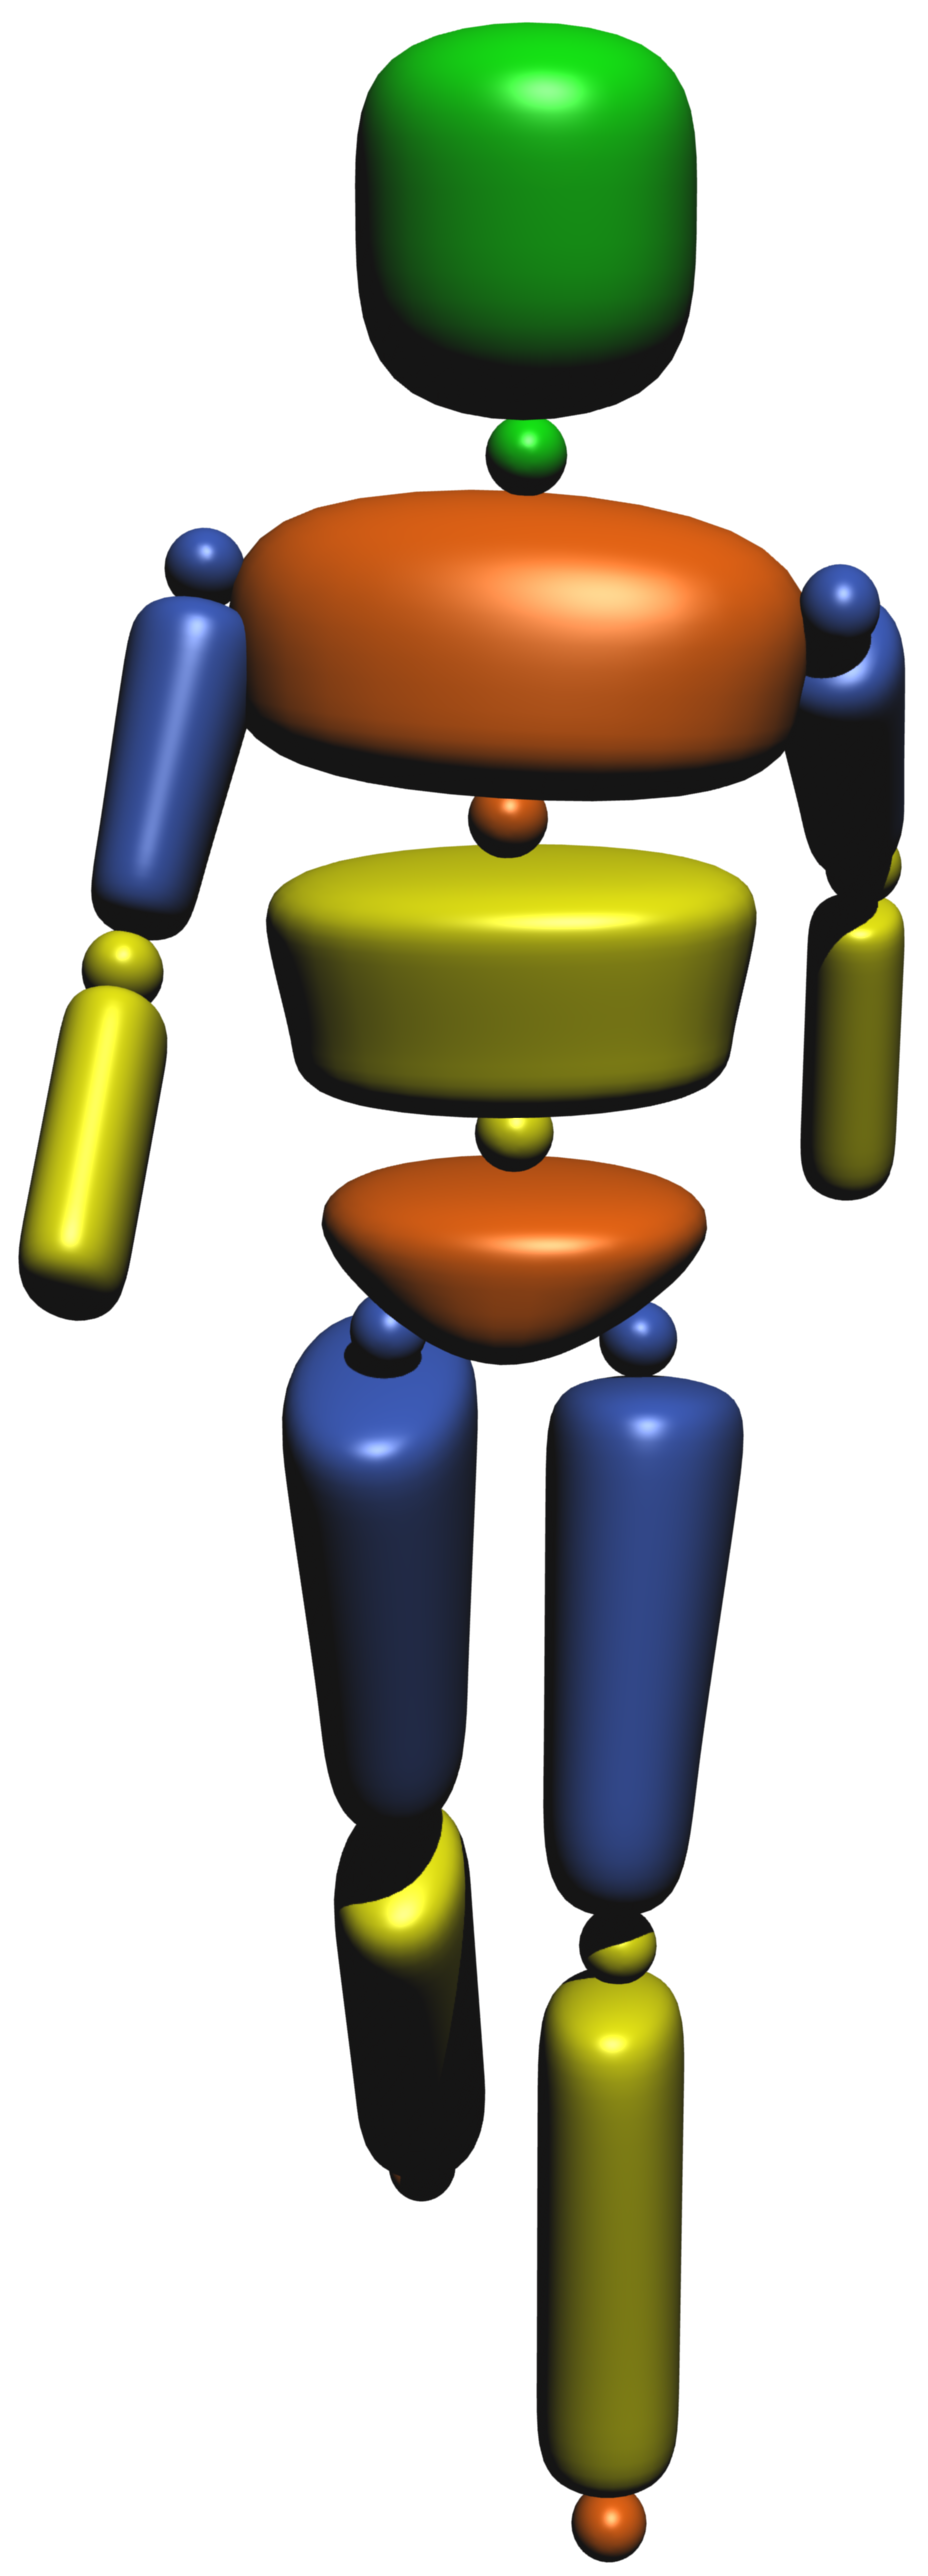
\includegraphics[width=0.1\textwidth]{fig/knubbi.png}
%   \caption{Example picture.}
%   \label{fig:knubbi}
%\end{figure}

% Table
%\begin{table}[h]
%\caption{Example table.}
%   \begin{tabularx}{0.48\textwidth}{llr}
%   		 \toprule 
%   		 Symbol & \multicolumn{1}{X}{Description} & Value [m] \\
%		 \midrule
%		  $A_x$ & Horizontal coordinate of A$^{*}$ & 0.0745 \\
%		  $A_z$ & Vertical coordinate of A$^{*}$ & 0.2650 \\  \noalign{\smallskip}
%		  
%		  $C_x$ & Horizontal coordinate of C$^{\#}$ & 0.0700 \\
%		  $C_z$ & Vertical coordinate of C$^{\#}$ & 0.1000 \\
%		  $D_x$ & Horizontal coordinate of D$^{\dag}$ & 0.0602 \\
%		  $D_z$ & Vertical coordinate of D$^{\dag}$ & 0.0860 \\
%		 \bottomrule
%   \end{tabularx}  \label{tab:initmodel}
%\end{table}